\subsection{Webmin}  

Webmin es una herramienta de administración de sistemas basada en la web muy popular para sistemas Unix-like, que incluye soporte para configurar y administrar varios servicios, entre ellos Bacula. Usar Webmin para administrar Bacula puede proporcionar varios beneficios, especialmente en términos de accesibilidad y facilidad de uso. A continuación, se detallan las razones para usar Webmin:

\begin{enumerate}
    \item \textbf{Accesibilidad}: Como interfaz basada en la web, Webmin permite a los administradores acceder a la configuración de Bacula desde cualquier lugar, solo necesitas un navegador web.
    \item \textbf{Usabilidad}: Webmin ofrece una interfaz de usuario gráfica intuitiva, lo que hace que sea más fácil para los usuarios que no están familiarizados con la línea de comandos.
    \item \textbf{Flexibilidad}: Permite gestionar no solo Bacula, sino también otros aspectos del sistema, lo que lo hace útil para administradores que desean una herramienta única para múltiples tareas.
    \item \textbf{Configuración simplificada}: Proporciona módulos que simplifican la configuración de las complejas opciones de Bacula, reduciendo el riesgo de errores.
    \item \textbf{Comunidad y soporte}: Tiene una gran base de usuarios y una comunidad activa que puede ofrecer soporte y consejos.
\end{enumerate}

Además webmin puede ser útil en la lucha contra el ransomware:
\begin{enumerate}
    \item \textbf{Actualizaciones del Sistema}: Webmin puede configurar y manejar actualizaciones automáticas para el sistema operativo y el software instalado, lo cual es crucial para protegerse contra vulnerabilidades conocidas que podrían ser explotadas por ransomware.
    \item \textbf{Gestión de Backups}: A través del módulo de Bacula u otros módulos de backup como el módulo de rsync, Webmin puede configurar políticas de backups regulares y seguras, esencial para la recuperación de datos en caso de un ataque de ransomware.
    \item \textbf{Control de Acceso y Seguridad}: Webmin permite configurar políticas de seguridad, como la gestión de permisos de usuarios, el uso de contraseñas seguras, y configuraciones de firewall. Establecer un control de acceso estricto puede ayudar a prevenir accesos no autorizados que podrían resultar en un cifrado malicioso de datos.
    \item \textbf{Monitoreo y Alertas}: Webmin proporciona módulos para el monitoreo del sistema que pueden ser configurados para alertar a los administradores sobre actividad sospechosa o no autorizada, un componente crucial en la detección temprana de ataques de ransomware u otras infracciones de seguridad.
    \item \textbf{Configuración de Servidores de Correo}: Configurar correctamente los servidores de correo para filtrar spam y mensajes maliciosos puede reducir el riesgo de phishing, que es uno de los vectores de ataque más comunes para la distribución de ransomware.
\end{enumerate}

Otras herramientas graficas comparadas con webmin:

\begin{table}[H]
    \centering
    \small
    \begin{tabularx}{\textwidth}{>{\centering\arraybackslash}p{0.2\textwidth}>{\centering\arraybackslash}p{0.24\textwidth}>{\centering\arraybackslash}p{0.24\textwidth}>{\centering\arraybackslash}X} 
        \hline
        \thead{Interfaz} & \thead{Webmin} & \thead{Bacula Web} & \thead{BAT} \\
        \hline
        Tipo de Interfaz &Basada en la web & Basada en la web & Aplicación de escritorio\\
        Accesibilidad	 & Acceso remoto a través del navegador web & Acceso remoto a través del navegador web & Local o remoto mediante X11 forwarding\\
        Configuración & Configuración simplificada mediante módulos GUI & Configuración y monitoreo visual de trabajos de backup &Gestión detallada de configuraciones de Bacula\\
        Monitoreo & Monitoreo básico de tareas y estado del sistema & Monitoreo avanzado de trabajos, incluyendo reportes & Monitoreo detallado y gestión de trabajos y dispositivos \\
        Integración del Sistema	&Alta, gestiona otros servicios del sistema & Específica para Bacula & Específica para Bacula \\
        Facilidad de Uso & Interfaz intuitiva y fácil de usar para administradores & Requiere algo de familiaridad con Bacula & Requiere conocimiento avanzado de Bacula\\
        Soporte y Documentación & Amplia documentación y soporte comunitario & Documentación limitada, soporte comunitario & Documentación técnica detallada, soporte limitado\\
        \bottomrule
    \end{tabularx}
    \caption{Comparación entre webmin y otras herramientas gráficas de bacula.}
\end{table}


\textbf{Instalación de Apache}
\medskip

Comenzamos por instalar Apache, que es necesario para Webmin.
\begin{verbatim}
apt install apache2
\end{verbatim}

\begin{figure}[H]
    \centering
    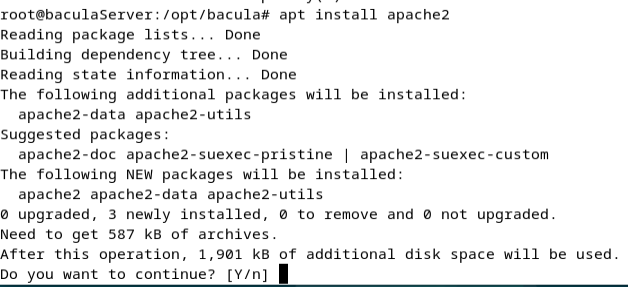
\includegraphics[width=0.5\linewidth]{instalacionBacula/apache2.png}
    \caption{Instalación de Apache2}
\end{figure}

\textbf{Configuración del Firewall}
\medskip

Agregamos las reglas necesarias en el firewall para permitir el tráfico HTTP y HTTPS.
\begin{verbatim}
sudo ufw allow 80/tcp
sudo ufw allow 443/tcp
\end{verbatim}

\begin{figure}[H]
    \centering
    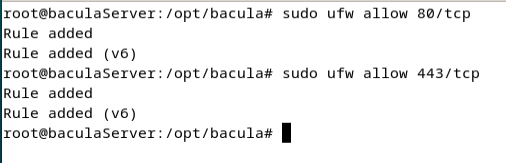
\includegraphics[width=0.5\linewidth]{instalacionBacula/htpsFirewall.png}
    \caption{Añadiendo reglas de HTTP y HTTPS al firewall}
\end{figure}

\textbf{Instalación de Webmin}
\medskip

Procedemos a descargar y ejecutar el script para configurar los repositorios de Webmin.
\begin{verbatim}
curl -o setup-repos.sh https://raw.githubusercontent.com/webmin/
webmin/master/setup-repos.sh sh setup-repos.sh
\end{verbatim}

\begin{figure}[H]
    \centering
    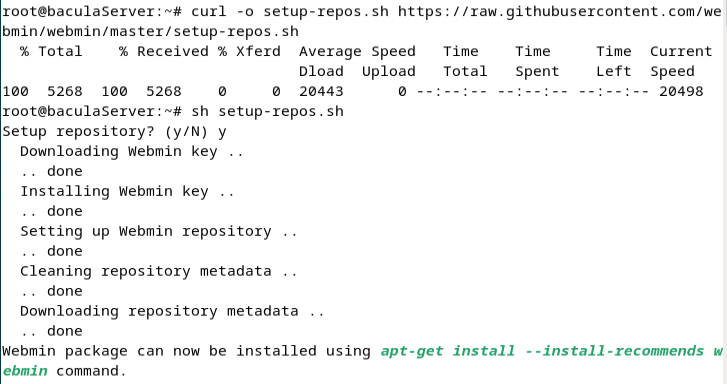
\includegraphics[width=0.5\linewidth]{instalacionBacula/CURLwebmin.png}
    \caption{Descargando y ejecutando el script de configuración de Webmin}
\end{figure}

Instalamos Webmin utilizando el gestor de paquetes apt.
\begin{verbatim}
apt-get install webmin --install-recommends
\end{verbatim}

\begin{figure}[H]
    \centering
    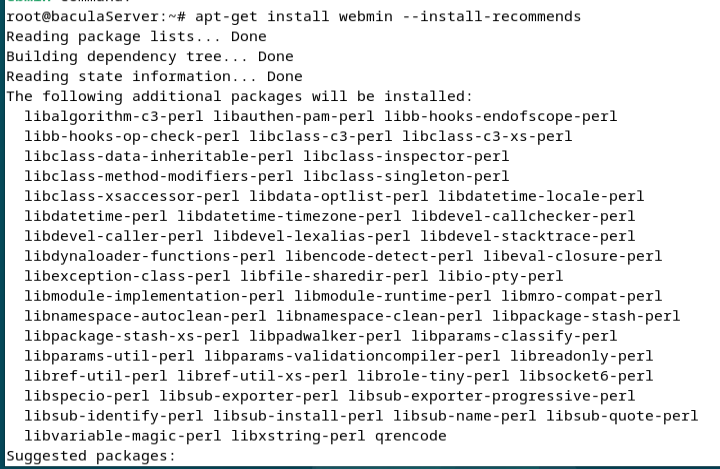
\includegraphics[width=0.5\linewidth]{instalacionBacula/instalWebminn.png}
    \caption{Instalación de Webmin}
\end{figure}

\textbf{Configuración del Puerto en el Firewall}
\medskip

Añadimos la regla en el firewall para permitir el tráfico en el puerto 10000, usado por Webmin.
\begin{verbatim}
sudo ufw allow 10000/tcp
\end{verbatim}

\begin{figure}[H]
    \centering
    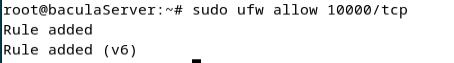
\includegraphics[width=0.5\linewidth]{instalacionBacula/puerto10000.png}
    \caption{Añadiendo el puerto de Webmin al firewall}
\end{figure}

\textbf{Acceso a la Interfaz de Webmin}
\medskip

Ahora podemos acceder a la interfaz de Webmin mediante un navegador web utilizando la dirección IP del servidor y el puerto configurado.

\begin{figure}[H]
    \centering
    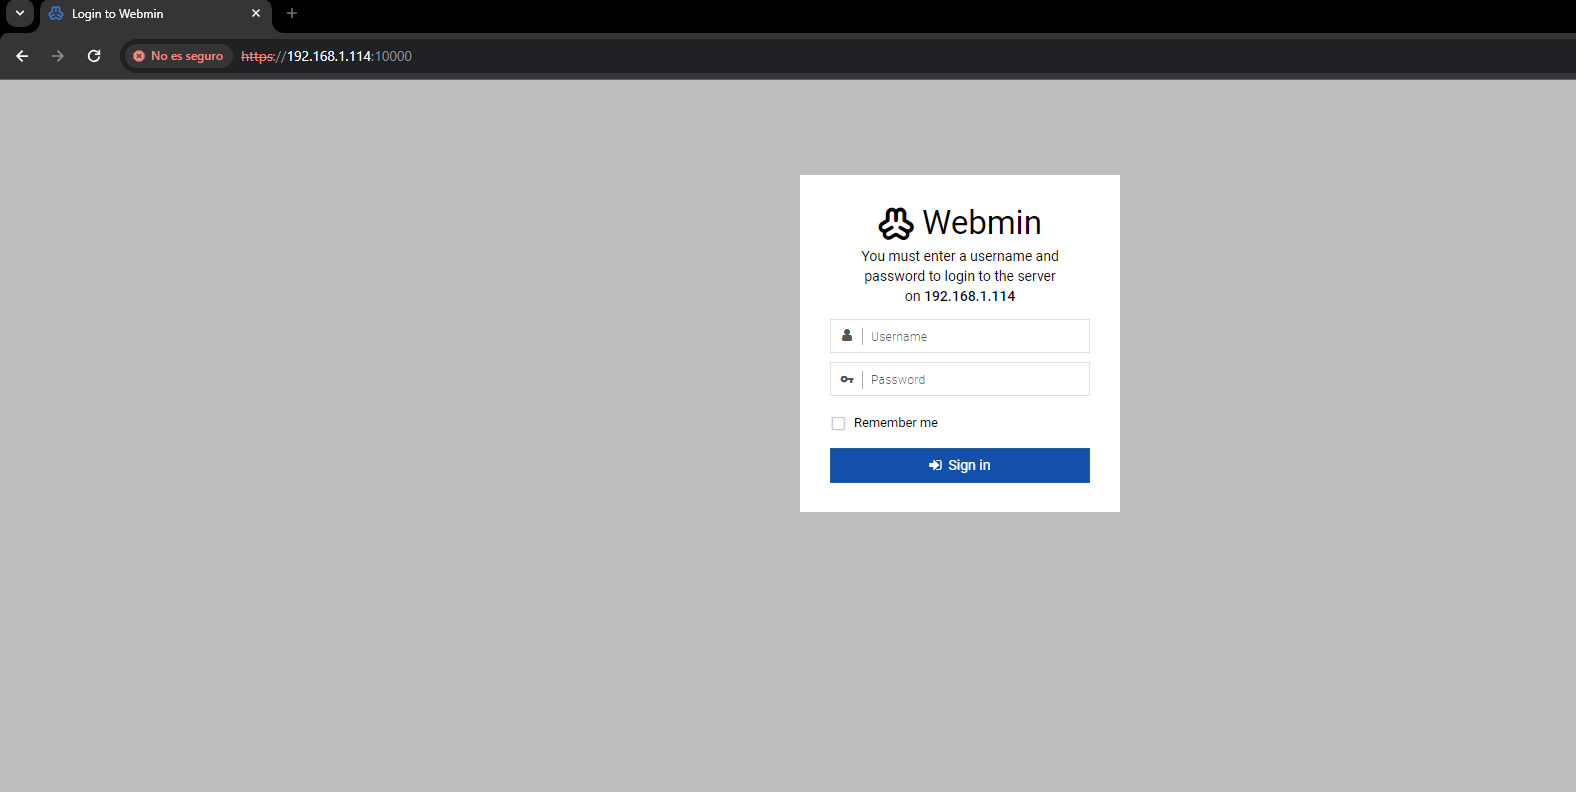
\includegraphics[width=0.5\linewidth]{instalacionBacula/webmin.png}
    \caption{Interfaz de acceso a Webmin}
\end{figure}

\textbf{Configuración del Módulo Bacula en Webmin}
\medskip

Configuramos el módulo Bacula en Webmin añadiendo las rutas necesarias para los comandos de Bacula.
% poner enumerate
\begin{verbatim}
Bacula configuration directory: /opt/bacula/etc
Full path to bextract command: /opt/bacula/bin/bextract
Full path to bls command: /opt/bacula/bin/bls
Full path to btape command: /opt/bacula/bin/btape
\end{verbatim}

\begin{figure}[H]
    \centering
    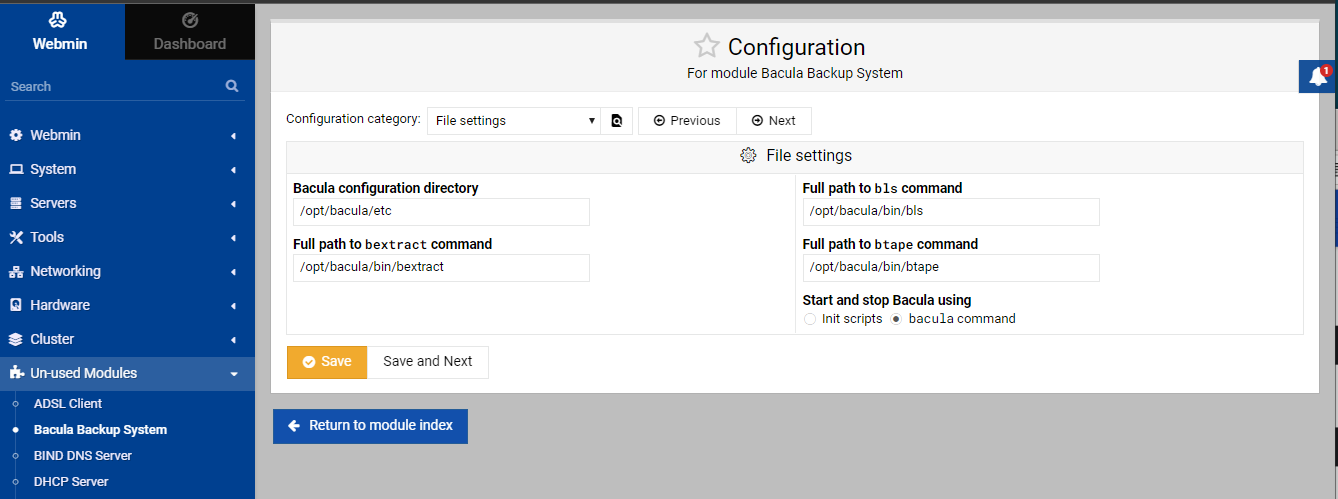
\includegraphics[width=0.5\linewidth]{instalacionBacula/pathwebmin.png}
    \caption{Configuración de los comandos de Bacula en Webmin}
\end{figure}

\textbf{Configuración de PostgreSQL para Bacula}\medskip

Si es necesario, ajustamos la configuración de PostgreSQL para permitir la autenticación del usuario de Bacula.
\begin{verbatim}
# TYPE  DATABASE        USER            ADDRESS                 METHOD
local   all             all                                     md5
\end{verbatim}

\begin{figure}[H]
    \centering
    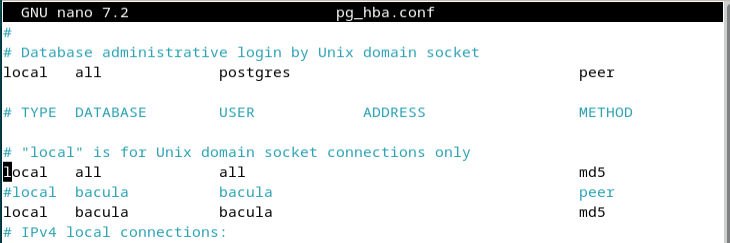
\includegraphics[width=0.5\linewidth]{instalacionBacula/md5postgesql.png}
    \caption{Configuración de PostgreSQL para Bacula}
\end{figure}

Reiniciamos el servicio de PostgreSQL para aplicar los cambios.
\begin{verbatim}
systemctl restart postgresql
\end{verbatim}
